\documentclass{webofc}
\usepackage[utf8]{inputenc}
\usepackage{xcolor}
\usepackage{minted}
\usepackage{tabto}
\usepackage{mathtools}

\title{Columnar data processing for HEP analysis}
\author{Jim Pivarski\inst{1} \and Jaydeep Nandi\inst{2} \and David Lange\inst{1} \and Peter Elmer\inst{1}}
\date{October 2018}

\abstract{FIXME}

%% \abstract{In the last stages of data analysis, only order-of-magnitude computing speedups translate into increased human productivity, and only if they're not difficult to set up. Producing a plot in a second instead of an hour is life-changing, but not if it takes two hours to write the analysis code. Fortunately, HPC-inspired techniques can result in such large speedups, but unfortunately, they can be difficult to use in a HEP setting.

%% These techniques generally favor operating on columns— arrays representing a single attribute across events, rather than whole events individually— which allows data to stream predictably from disk media to main memory and finally to CPU/GPU/KNL onboard memory (e.g. L* cache) for prefetching and sometimes allows for for vectorization. However, the need to work with variable-length structures in HEP, such as different numbers of particles per event, makes it difficult to apply this technique to HEP problems.

%% We will describe several new software tools to make it easier to compute analysis functions with columnar arrays in HEP: array-at-a-time I/O in ROOT ("BulkIO") and Python/Numpy ("uproot"), compiling object-oriented analysis code into columnar operations ("oamap" for "object-array mapping"), and storage solutions with columnar granularity. We will show performance plots and usage examples.}

\xdefinecolor{dianablue}{rgb}{0.18,0.24,0.31}
\xdefinecolor{darkblue}{rgb}{0.1,0.1,0.7}
\xdefinecolor{darkgreen}{rgb}{0,0.5,0}
\xdefinecolor{darkgrey}{rgb}{0.35,0.35,0.35}
\xdefinecolor{darkorange}{rgb}{0.8,0.5,0}
\xdefinecolor{darkred}{rgb}{0.7,0,0}
\definecolor{darkgreen}{rgb}{0,0.6,0}
\definecolor{mauve}{rgb}{0.58,0,0.82}

\definecolor{mycolor}{HTML}{FF6600}
\definecolor{cppcolor}{HTML}{00AAD4}
\definecolor{rootcolor}{HTML}{2A2AFF}
\definecolor{rootnpcolor}{HTML}{008000}
\definecolor{pythoncolor}{HTML}{FF00CC}

\begin{document}
\institute{Princeton University \and National Institute of Technology, Silchar, India}

\maketitle

\section{Introduction}

The field of High Energy Physics (HEP) has always dealt with big data, large enough datasets that finite memory and processing speed cannot be ignored. Traditionally, physicists have relied on compiled languages like Fortran and C++ to analyze large datasets in batch, but this limits interactive exploration. Today, data analysts in other fields, including industry, are developing tools to analyze large datasets in high-level languages, but these tools treat data as rectangular tables and flat arrays. HEP analysis requires {\it nested} data--- arbitrarily many tracks within jets or variable-sized collections of particle candidates--- which do not fit into rectangular data without padding and truncation.

This paper introduces awkward-array, a library designed to extend the array programming model used by MATLAB, R, Numpy, and Pandas to nested and otherwise ``awkward'' data structures. The library is written in pure Python, depending only on Numpy, for easier integration into the Python data science ecosystem.

\section{Array programming and its extension to nested data}

Array programming is an interface in which individual user commands apply to whole arrays: each function call performs a regular operation on millions of data points. Pioneered by APL in 1963, this programming style appears primarily in analyst-facing data processing languages such as S~(1976), MATLAB~(1984), S-PLUS~(1988), R~(1993), and Numpy~(2005). Beyond its succinct syntax, which can be easier to read than the corresponding for-loops, it encourages simple passes over columnar data that facilitates CPU cache-prefetching and vectorization. In fact, programs written in an array programming style are also appropriately organized for Single Instruction Multiple Data (SIMD) processing, which makes it easier to migrate to GPUs.

Array programming usually includes the following elements (expressed in Numpy syntax here):

\begin{description}
\item[\hspace{1 cm}$\bullet$] Multidimensional slices: \tabto{5.8 cm}{\small \mintinline{python}{rgb_pixels[0, 50:100, ::3]}}
\item[\hspace{1 cm}$\bullet$] Elementwise operations: \tabto{5.8 cm}{\small \mintinline{python}{all_pz = all_pt * sinh(all_eta)}}
\item[\hspace{1 cm}$\bullet$] Broadcasting: \tabto{5.8 cm}{\small \mintinline{python}{all_phi - 2*pi}}
\item[\hspace{1 cm}$\bullet$] Array reduction: \tabto{5.8 cm}{\small \mintinline{python}{array.sum()}} $\to$ scalar
\item[\hspace{1 cm}$\bullet$] Masking (list compaction): \tabto{5.8 cm}{\small \mintinline{python}{data[trigger & (pt > 40)]}}
\item[\hspace{1 cm}$\bullet$] Fancy indexing (``gather''): \tabto{5.8 cm}{\small \mintinline{python}{all_eta[argsort(all_pt)]}}
\item[\hspace{1 cm}$\bullet$] Row/column commutativity \tabto{5.8 cm}{\small \mintinline{python}{table["column"][7]} (row 7 of column array)}
\tabto{5.8 cm}{\small \mintinline{python}{table[7]["column"]} (field of row tuple 7)}
\end{description}

\noindent The semantics of each of these is well established for rectangular tables and flat arrays, but they can be extended to arbitrarily nested data structures. The examples below illustrate common cases that are defined in detail later in the text. In these examples, {\small\mintinline{python}{events["jets"]}}, {\small\mintinline{python}{jetpt}}, etc., contain lists of arbitrarily many objects or values.

\begin{description}
\item[\hspace{1 cm}$\bullet$] Multidimensional slices: \tabto{5.8 cm}{\small \mintinline{python}{events["jets"][:, 0]}} $\to$ first jet per event
\item[\hspace{1 cm}$\bullet$] Elementwise operations: \tabto{5.8 cm}{\small \mintinline{python}{jetpt * sinh(jeteta)}} $\to$ keep nested structure
\item[\hspace{1 cm}$\bullet$] Broadcasting: \tabto{5.8 cm}{\small \mintinline{python}{jetphi - metphi}} $\to$ expand {\small \mintinline{python}{metphi}} from
\tabto{5.8 cm}one-per-event to one-per-jet before operation
\item[\hspace{1 cm}$\bullet$] Array reduction: \tabto{5.8 cm}{\small \mintinline{python}{jetpt.max()}} $\to$ array of max jet $p_T$ per event
\item[\hspace{1 cm}$\bullet$] Masking (list compaction): \tabto{5.8 cm}{\small \mintinline{python}{data[trigger]}} $\to$ drop whole events
\tabto{5.8 cm}{\small \mintinline{python}{data[jetpt > 40]}} $\to$ drop jets from events  
\item[\hspace{1 cm}$\bullet$] Fancy indexing (``gather''): \tabto{5.8 cm}{\small \mintinline{python}{a = argmax(jetpt)}} $\to$ {\small \mintinline{python}{[[2], [], [1], [4]]}}
\tabto{5.8 cm}{\small \mintinline{python}{jeteta[a]}} $\to$ \mbox{\small \mintinline{python}{[[3.6], [], [-1.2], [0.4]]}\hspace{-0.5 cm}}
\item[\hspace{1 cm}$\bullet$] Row/column commutativity \tabto{5.8 cm}{\small \mintinline{python}{events["jets"]["pt"][7, 1]}} is the same as
\tabto{5.8 cm}{\small \mintinline{python}{events["jets"][7]["pt"][1]}} and \\
\tabto{5.8 cm}{\small \mintinline{python}{events["jets"][7, 1]["pt"]}} etc.
\end{description}

\noindent Consider the following extended example, which generates particle candidate combinations and then selects the best one. Procedural code like this (Python syntax):

{\small\begin{minted}{python}
leptoquarks = []
for event in dataset:
    best = None
    for jet in event.jets:
        for lepton in event.leptons:
            if cut(jet, lepton):
                leptoquark = jet + lepton        # Lorentz vector + operator
                if best is None or quality(leptoquark) > quality(best):
                    best = leptoquark
    if best is not None:
        leptoquarks.append(best)
\end{minted}
}

\noindent can be replaced by the following array-centric script.

{\small\begin{minted}{python}
pairs = events["jets"].cross(events["leptons"])  # cross-join within events
goodpairs = pairs[cut(pairs["0"], pairs["1"])]   # into pairs["0"] and ["1"]
candidates = pairs["0"] + pairs["1"]             # Lorentz vector + operator
best = candidates[quality(candidates).argmax()]  # best indexes, then objects
leptoquarks = best.flatten()                     # reduce to flat array
\end{minted}
}

\section{High-level types and array programming interface}

Arrays introduce a degree of static typing to dynamically typed programming languages, in the sense that all elements of an array have the same type and an operation may be performed across all elements without expensive type-checks. Conventional array processing environments like Numpy only support primitive types: numbers, booleans, and other fixed-size values (including records of fixed-size values). Fixed-size subarrays are presented as an array's multidimensional ``shape,'' and may be considered part of the type. Introducing nested data requires additional data types.

The type of a flat array with length $n$ could be denoted $[0, n) \to P$, as a function signature that takes integers between $0$ (inclusive) and $n$ (exclusive) to a primitive type $P$. An array of length $n$ with variable-sized subarrays would be $[0, n) \to [0, \infty) \to P$, as any non-negative integer could be in the second domain (though some are not valid for a particular dataset). This is known as a jagged, or ragged, array. Jagged arrays may be nested: $[0, n) \to [0, \infty) \to [0, \infty) \to P$.

The extension of multidimensional slices to $[0, \infty)$ should be clear--- instead of selecting from $0$ to $n$ slots, slices select from $0$ to a number of slots that only becomes known while iterating through the array. (The type-safety is weaker than for flat arrays, whose shape is fully known in constant time.) Elementwise operations are only possible if all subarrays in each argument have the same lengths, and they preserve that structure in the output.

Conventional broadcasting allows scalar $P$ data to be included in elementwise operations with arrays $[0, n) \to P$ by duplicating the one scalar to $n$ array elements. Jagged broadcasting duplicates each element of a flat array $[0, n) \to P$ to the corresponding jagged array elements $[0, n) \to [0, \infty) \to P$, increasing the depth of jaggedness by one. The same applies for any depth of jaggedness to one level deeper.

When filtering a jagged array with a mask, we may want to remove subarrays (representing events) or we may want to remove subarray elements (representing particles). We can make that distinction by contrasting a boolean mask $[0, n) \to \mbox{\small\tt bool}$ with a jagged boolean mask $[0, n) \to [0, \infty) \to \mbox{\small\tt bool}$. In keeping with the rules of conventional array programming, a boolean mask would remove subarrays from a jagged array $[0, n) \to [0, \infty) \to P$. Extending these rules, a jagged boolean mask could remove subarray elements if they have the same jagged structure.

Similarly, an integer array $[0, m) \to \mbox{\small\tt int}$ selects $m$ subarrays from a jagged array by the conventional rules, but a jagged integer array $[0, n) \to [0, \infty) \to \mbox{\small\tt int}$ could select subarray elements. Since this ``gather'' feature is often used with functions like {\it argmax}, {\it argmin}, and {\it argsort} to identify important indexes in one array and select elements at those indexes from another array, the jagged {\it argmax} and {\it argmin} should return jagged arrays with zero or one element in each subarray--- the max or min if any elements exist.

Tables with named, differently typed columns can be included in this type system as a mapping from names to types. For instance,

\[ [0, n) \to \left\{\begin{array}{l c l}
\mbox{\small\tt "one"} & \to & P_1 \\
\mbox{\small\tt "two"} & \to & P_2 \\
\mbox{\small\tt "three"} & \to & P_3\mbox{.} \end{array}\right. \]

\noindent In our extension of array programming, tables and jaggedness can be composed. This is useful in HEP for describing event records that contain variable-sized lists of particles, each with a different multiplicity, each containing attributes of various types. In some cases, it's useful for the particle attributes to be variable-sized lists as well. Type descriptions may be arbitrary trees:

\[ [0, n) \to [0, \infty) \to \left\{\begin{array}{l c l}
\mbox{\small\tt "one"} & \to & [0, m) \to \left \{\begin{array}{l c l} \mbox{\small\tt "x"} & \to & [0, \infty) \to P_1 \\ \mbox{\small\tt "y"} & \to & P_2 \end{array}\right. \\
\mbox{\small\tt "two"} & \to & P_3 \\
\mbox{\small\tt "three"} & \to & P_4\mbox{.} \end{array}\right. \]

Rectangular tables may be sliced by row (integer index) or column (string index). So can jagged tables. A table described by $[0, n) \to [0, \infty) \to \{\mbox{\small\tt "one"} \to T_1\mbox{, }\mbox{\small\tt "two"} \to T_2\}$ sliced by a string index {\small\tt "one"} returns a jagged array $[0, n) \to [0, \infty) \to T_1$. In general, this means that integer indexes commute with string indexes, though integer indexes do not commute with other integer indexes, nor do string indexes commute with other strings.

Primitives, variable-sized lists, and tables of records would be sufficient for most HEP cases, but sometimes polymorphic types and cross-references (pointers) are needed. Polymorphic types can be included with unions $T = T_1\ |\ T_2$ (elements may be type $T_1$ or type $T_2$) and optional types $?T$ (elements may be type $T$ or null). Since the possibilities of a polymorphic type are enumerated, operations must be legal on all enumerated possibilities, and operations on an optional type are only applied to non-null elements.

For cross-references, such as tagging jets with their associated leptons, we allow type trees to be arbitrary graphs. A list may contain elements of a list elsewhere in the graph or its own ancestors. As an example of the latter case,

\[ [0, n) \to T \coloneqq \big( \mbox{\small\tt int}\ \big|\ [0, \infty) \to T \big) \]

\noindent is an array that may contain integers, lists of integers, or any depth of lists of integers.

This set of types is as inclusive as most high-level programming languages, and it can be constructed entirely from columnar arrays.

\section{Low-level data structures and their uses}

The fundamental construct for variable-sized, nested structure is the jagged array. To represent a list of unequal-length sublists with the following logical structure, we store the flattened content in one array and the structure in either an ``offsets'' or a ``parents'' array.

\vspace{\baselineskip}
Logical structure: \tabto{4 cm}{\ttfamily\textcolor{black}{[\textcolor{red}{[}\textcolor{darkblue}{0, 1, 2}], \textcolor{red}{[}], \textcolor{red}{[}\textcolor{darkblue}{3, 4}], \textcolor{red}{[}\textcolor{darkblue}{5, 6, 7, 8}], \textcolor{red}{[}]\ \ \textcolor{red}{]}}}

\vspace{0.05 cm}
Content:           \tabto{4 cm}{\ttfamily\verb|[ |\textcolor{darkblue}{0, 1, 2}\verb|,       |\textcolor{darkblue}{3, 4}\verb|,   |\textcolor{darkblue}{5, 6, 7, 8}\verb|]|}

\vspace{0.05 cm}
Offsets:           \tabto{4 cm}{\ttfamily\verb|[|\textcolor{red}{0,}\verb|         |\textcolor{red}{3,}\verb|  |\textcolor{red}{3,}\verb|      |\textcolor{red}{5,}\verb|            |\textcolor{red}{10, 10}\verb|]|}

\vspace{0.05 cm}
Parents:           \tabto{4 cm}{\ttfamily\verb|[ |\textcolor{darkgreen}{0, 0, 0}\verb|        |\textcolor{purple}{2, 2,}\verb|   |\textcolor{darkorange}{3, 3, 3, 3}\verb|]|}

\vspace{\baselineskip}
The offsets array may be constructed as the content index after every opening bracket (the ``starts'' array) appended by the total length, or it may be constructed as the content index after every closing bracket (the ``stops'' array) prepended by zero. It is useful for descending from outer levels to inner levels of structure.

The parents array has the same length as the contents array; it associates each content element with the index of the subarray that contains it. A parents array is incapable of expressing empty sublists at the end of a list (as in the above example), but it can specify empty lists in a sequence by skipping integers. Offsets are therefore more general than parents, but parents are useful in reducer operations that ascend from inner levels to outer levels of structure. 

The awkward-array library has a {\tt\small JaggedArray} implementation that allows arbitrary contents--- nesting a {\tt\small JaggedArray} within a {\tt\small JaggedArray} constructs $[0, n) \to [0, \infty) \to [0, \infty) \to P$. The {\tt\small JaggedArray.\_\_getitem\_\_} method overrides square brackets in Python to provide slicing, masking, and fancy indexing with all the features described in the previous section. Elementwise operations and broadcasting are implemented in {\tt\small \_\_array\_ufunc\_\_}, which overrides the behavior of all universal functions in Numpy.

Tables of records are implemented as a {\tt\small Table} class that maps column names to arrays. This is like Numpy's ``record arrays,'' except that a Numpy record array must be a contiguous array of structs, while awkward-array's {\tt\small Table} may be non-contiguous or a struct of arrays. {\tt\small JaggedArray} and {\tt\small Table} interact to let integer and string valued indexes commute, which hides the arrays-of-structs/structs-of-arrays distinction.

{\tt\small UnionArray} and {\tt\small MaskedArray} implement polymorphism and optional types. Numpy has a masked array type, but {\tt\small MaskedArray} shares conventions with the rest of awkward-array's suite and additionally has a {\tt\small BitMaskedArray} variant for compatibility with Apache Arrow (next section).

In HEP applications, it is useful to have datasets representing arrays of objects, such as $[0, n) \to \mbox{\tt\small LorentzVector}$, which returns \mbox{\tt\small LorentzVector} objects when given an index. Numpy has an ``object array'' type, which stores pointers to Python objects in memory, but awkward-array's {\tt\small ObjectArray} constructs a Python object when given an index. This allows us to represent such data with 12$\times$ less memory, as we will see in the section on performance below.

In the same spirit as integer/string index commutivity, methods of objects returned by {\tt\small ObjectArray} may be applied to the entire array for vectorized HEP calculations. For instance, an {\tt\small ObjectArray} of \mbox{\tt\small LorentzVectors} may be boosted en masse:

\begin{center}
\tt\small subleading\_jets.boost(leading\_jets)
\end{center}

\noindent which works equally well if {\tt\small subleading\_jets} is a jagged array (several per event) and {\tt\small leading\_jets} is a flat array (one per event), thanks to jagged broadcasting. An array of strings is an {\tt\small ObjectArray} of a {\tt\small JaggedArray}, converting subarrays of characters into {\tt\small str} objects on demand.

In addition, awkward-array provides some array classes for dealing with data structures without affecting their high-level data types. Some file formats provide data in discontiguous chunks, such as ROOT's baskets or Parquet's pages and row groups. {\tt\small ChunkedArray} lets us view discontiguous chunks of data as a single logical array without copying, by mapping indexes. {\tt\small VirtualArray} uses a given function to generate an array on demand, rather than holding it in memory (passing it to a temporary cache, if desired). A chunked, virtual array is a lazy array, like Dask's ``delayed arrays.''

Any of these can be cross-referenced Python objects, as the implementation is careful to avoid infinite recursion. To cross-reference individual elements, such as associating a single lepton with a jet, {\tt\small IndexedArray} represents a deferred indirection. An {\tt\small index} array stores locations {\tt\small j[i]} to look up in a {\tt\small content} array: given {\tt\small i}, it returns {\tt\small content[j[i]]}. {\tt\small JaggedArray} is like {\tt\small IndexedArray} except that it represents ranges of {\tt\small content} indexes, rather than individual indexes.

{\tt\small SparseArray} is the conceptual opposite of {\tt\small IndexedArray}: its {\tt\small index} and {\tt\small content} must be the same length and each {\tt\small index} is the logical position of the corresponding {\tt\small content}. Other indexes are presumed to be zero or some default value. As a sparse matrix, this is known as the COOrdinate format. Whereas an {\tt\small IndexedArray} represents a smaller logical array than its {\tt\small content} (or one with duplicates), a {\tt\small SparseArray} represents a larger logical array than its {\tt\small content}. It is useful in HEP for looking up indexes in a table that is far too large to fit in memory, such as a mapping from ten-digit detector identifiers to measurement corrections.

\section{Persistence, ROOT and Apache Arrow compatibility}

blah blah blah

\section{Performance measurements}

blah blah blah

\begin{table}[b]
\begin{minipage}{0.4\linewidth}\scriptsize
\begin{tabular}{r p{0.9\linewidth}}
\underline{MB} & \underline{RAM memory occupied by data} \\
& \\
311.95 & \textcolor{pythoncolor}{Python list of lists of dicts} \\
215.11 & \textcolor{rootnpcolor}{root\_numpy's array of arrays} \\
139.79 & \textcolor{pythoncolor}{Python list of lists of {\tt \_\_slots\_\_} classes} \\
& \\
 37.19 & \textcolor{gray}{serialized JSON text} \\
& \\
 22.38 & \textcolor{cppcolor}{{\tt\scriptsize std::vector<std::vector<struct>>}} \\
& \\
 11.67 & \textcolor{mycolor}{JaggedArray of Table of pt, eta, phi} \\
%% & \\
%% & \textcolor{gray}{\scriptsize 1 MB = 1024$^2$ bytes} \\
%% & \textcolor{gray}{\scriptsize 701,716 events containing 552,056 muons} \\
%% & \textcolor{gray}{\scriptsize storing pt, eta, phi as float32} \\
\end{tabular}

\vspace{1.35 cm}
\end{minipage}\begin{minipage}{0.6\linewidth}{\mbox{\hspace{-3.5 cm}\begin{minipage}{1.5\linewidth}\scriptsize
\begin{tabular}{p{0.83\linewidth} l}
\hfill \underline{time to complete load, compute, or both} & \underline{sec} \\
& \\
\hfill \textcolor{rootcolor}{PyROOT load and compute} & 45.9 \\
\hfill \textcolor{mycolor}{JaggedArray compute in Python for loops} & 13.4 \\
& \\
\hfill \textcolor{rootnpcolor}{root\_numpy compute in loop over ufuncs} & \ 1.96 \\
\hfill \textcolor{pythoncolor}{Python list of lists of dicts in Python for loops} & \ 1.24 \\
\hfill \textcolor{pythoncolor}{Python list of lists of {\tt \_\_slots\_\_} classes in Python for loops} & \ 1.23 \\
\hfill \textcolor{rootnpcolor}{root\_numpy load} & \ 0.635 \\
& \\
\hfill \textcolor{rootcolor}{ROOT RDataFrame load and compute} & \ 0.163 \\          % -O0: 0.326, -O1: 0.172, -O2: 0.162, -O3: 0.163
\hfill \textcolor{rootcolor}{ROOT TTreeReader load and compute} &  \ 0.091 \\        % -O0: 0.164, -O1: 0.071, -O2: 0.091, -O3: 0.091
\hfill \textcolor{rootcolor}{ROOT TBranch::GetEntry load and compute} & \ 0.046 \\   % -O0: 0.052, -O1: 0.049, -O2: 0.049, -O3: 0.046
\hfill \textcolor{mycolor}{uproot load} & \ 0.031 \\
\hfill \textcolor{mycolor}{JaggedArray compute as Numpy-like ufunc} & \ 0.023 \\
\hfill \textcolor{mycolor}{JaggedArray compute in Numba-accelerated Python for loops} & \ 0.023 \\
%% & \\
%% \hfill \textcolor{gray}{\scriptsize all with warmed disk cache in the same environment} & \\
\end{tabular}
\end{minipage}}}\end{minipage}
\caption{\label{quantify}}
\end{table}

%% \begin{minted}{python}
%% def cross(self, other):
%%     offsets = counts2offsets(self.counts * other.counts)
%%     parents = offsets2parents(offsets)
%%     indexes = numpy.arange(offsets[-1], dtype=int)

%%     # fancy indexing get -> SIMD gather
%%     ocp = other.counts[parents]
%%     iop = indexes - offsets[parents]
%%     iop_ocp = iop // ocp

%%     left = self.content[self.starts[parents] + iop_ocp]
%%     right = other.content[other.starts[parents] + iop - ocp * iop_ocp]

%%     return JaggedArray.fromoffsets(offsets, Table(left, right))
%% \end{minted}

%% \begin{figure}
%% \begin{center}
%% 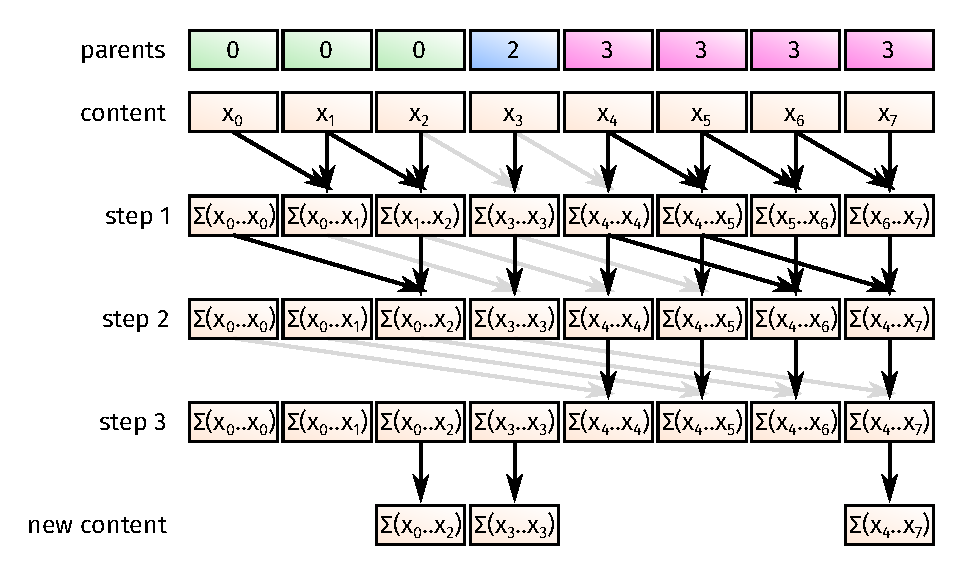
\includegraphics[width=0.7\linewidth]{hillis-steele-3.pdf}
%% \end{center}

%% \caption{\label{hillis-steele-3}}
%% \end{figure}

\begin{figure}
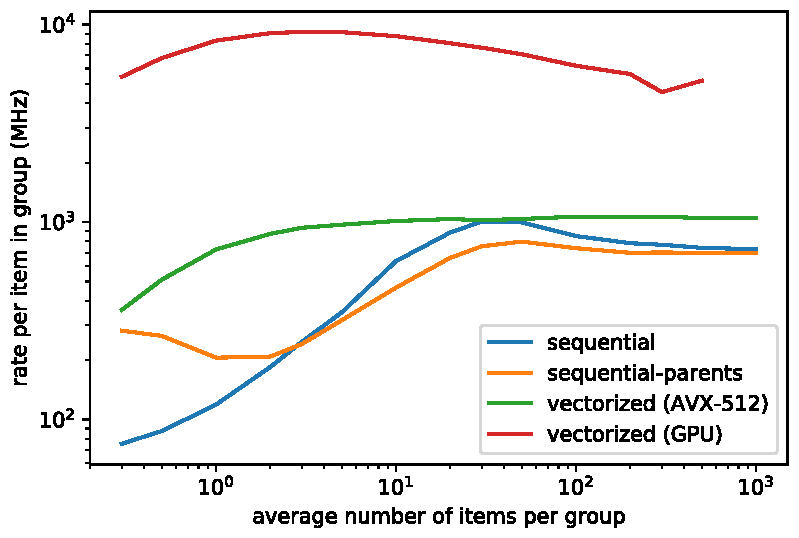
\includegraphics[width=0.5\linewidth]{sum_rates_logy.pdf}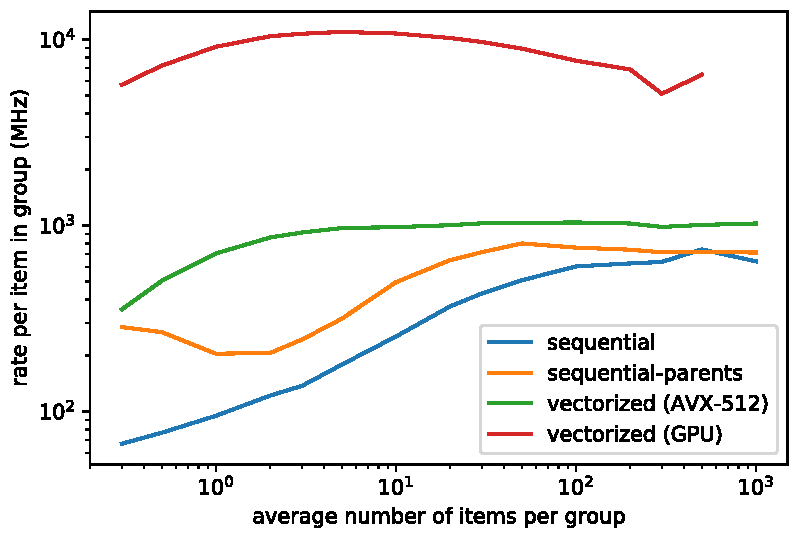
\includegraphics[width=0.5\linewidth]{max_rates_logy.pdf}

\caption{\label{rates_logy}}
\end{figure}

\section{Future directions}

Numba, Pandas, Dask, GPU

\section{Acknowledgements}

This work was supported by the National Science Foundation under grants ACI-1450377 and PHY-1624356.

\begin{thebibliography}{8}
% Journal Author, Journal \textbf{Volume}, page numbers (year)

\bibitem{uproot} Jim Pivarski et al., ``uproot'' [software], Release 3.2.6, Zenodo, 22 October, 2018. \url{https://zenodo.org/record/1469102}

\bibitem{uproot-methods} Jim Pivarski et al., ``uproot-methods'' [software], Release 0.4.1, Zenodo, 26 October, 2018. \url{https://zenodo.org/record/1472439}

\bibitem{awkward} Jim Pivarski, ``awkward-array'' [software], Release 0.4.1, Zenodo, 26 October, 2018. \url{https://zenodo.org/record/1472437}

\bibitem{ieee} FIXME: IEEE paper

\bibitem{columnar-objects} FIXME: columnar objects paper (find it in Strange Loop)

\end{thebibliography}

%%%%%%%%%%%%%%%%%%%%%%%%%%%%%%%%%%%%%%%%%%%%%%%%%%%%%%%%%%%%%%%


%% \begin{frame}[fragile]{Extension to variable-sized, nested structures}
%% \vspace{0.5 cm}

%% \vspace{0.5 cm}
%% \uncover<2->{A ``jagged array'' (content $+$ offsets and/or content $+$ parents) is a basic building block of variable-sized, nested structure.}

%% \begin{itemize}
%% \item<3-> use a jagged array as the content of another jagged array to get {\tt\small list<list<X>>}
%% \item<4-> use a fixed-size rectangular array of dimension {\tt\small N} as content to get {\tt\small list<X[N]>}
%% \item<5-> use a fixed-size rectangular array of dimension {\tt\small M} as offsets to get {\tt\small list<X>[M]}
%% \end{itemize}

%% \vspace{0.25 cm}
%% \uncover<6->{When combined with a table type (column names $\to$ arrays), this is as expressive as any combination of {\tt\small std::vector} and {\tt\small struct} (i.e.\ as expressive as ProtoBuf).}
%% \end{frame}

%% \begin{frame}{Array programming can be extended to jagged arrays}
%% \vspace{0.1 cm}
%% \begin{columns}
%% \column{1.05\linewidth}
%% \begin{itemize}\setlength{\itemsep}{0.15 cm}
%% \item Multidimensional slices: \tabto{5.5 cm}{\small \mintinline{python}{events["jets"][:, 0]}} $\to$ first jet per event
%% \item<2-> Elementwise operations: \tabto{5.5 cm}{\small \mintinline{python}{jetpt * sinh(jeteta)}} $\to$ \mbox{keep jagged structure\hspace{-1 cm}}
%% \item<3-> Broadcasting: \tabto{5.5 cm}{\small \mintinline{python}{jetphi - metphi}} $\to$ expand {\small \mintinline{python}{metphi}} from

%% \tabto{5.5 cm}one-per-event to one-per-jet before operation

%% \item<4-> Masking (list compaction): \tabto{5.5 cm}{\small \mintinline{python}{data[trigger]}} $\to$ drop whole events

%% \tabto{5.5 cm}{\small \mintinline{python}{data[jetpt > 40]}} $\to$ drop jets from events

%% \item<5-> Fancy indexing (gather/scatter): \tabto{5.5 cm}{\small \mintinline{python}{a = argmax(jetpt)}} $\to$ \mbox{\small \mintinline{python}{[[2], [], [1], [4]]}\hspace{-0.5 cm}}

%% \tabto{5.5 cm}{\small \mintinline{python}{jeteta[a]}} $\to$ \mbox{\small \mintinline{python}{[[3.6], [], [-1.2], [0.4]]}\hspace{-0.5 cm}}

%% \item<6-> Row/column commutativity \tabto{5.5 cm}{\small \mintinline{python}{events["jets"]["pt"][7, 1]}} \mbox{(all the same)\hspace{-0.5 cm}}

%% (project jagged tables to \tabto{5.5 cm}{\small \mintinline{python}{events["jets"][7]["pt"][1]}}

%% jagged arrays before indexing): \tabto{5.5 cm}{\small \mintinline{python}{events[7]["jets"]["pt"][1]}}

%% \tabto{5.5 cm}{\small \mintinline{python}{events["jets"][7, 1]["pt"]}}

%% \tabto{5.5 cm}{\small \mintinline{python}{events[7]["jets"][1]["pt"]}}

%% \item<7-> Jagged array reduction: \tabto{5.5 cm}{\small \mintinline{python}{jetpt.max()}} $\to$ array of max jet $p_T$ per event
%% \end{itemize}
%% \end{columns}
%% \end{frame}

%%%%%%%%%%%%%%%%%%%%%%%%%%%%%%%%%%%%%%%%%%%%%%%%%%%%%%%%%%%%%%%

%% \section{Appendix}
%% \tiny

%% \begin{minted}{python}
%% %%timeit
%% k = 0
%% for event in events:
%%     for muon in event:
%%         pz[k] = muon.pt * math.sinh(muon.eta)
%%         k += 1
%% \end{minted}

%% \begin{minted}{python}
%% import numba

%% @numba.jit
%% def callme(pz, events):
%%     k = 0
%%     for event in events:
%%         for muon in event:
%%             pz[k] = muon.pt * math.sinh(muon.eta)
%%             k += 1

%% %%timeit
%% callme(pz, events)
%% \end{minted}

%% \begin{minted}{python}
%% import numpy

%% %%timeit
%% pz = events["pt"] * numpy.sinh(events["eta"])
%% \end{minted}

%% \begin{minted}{python}
%% %%timeit
%% k = 0
%% for event in events:
%%     pt = event["Muon_pt"]
%%     eta = event["Muon_eta"]
%%     pz[k : k + len(pt)] = pt * numpy.sinh(eta)
%%     k += len(pt)
%% \end{minted}

%% \begin{minted}{python}
%% from math import sinh

%% events = [
%%     [],
%%     [{"pt": 129.8,
%%       "eta": -1.006,
%%       "phi": -0.581},
%%      {"pt": 73.08,
%%       "eta": -0.719,
%%       "phi": -1.51}],
%%     ...
%%     ]

%% %%timeit
%% k = 0
%% for event in events:
%%     for muon in event:
%%         pz[k] = (muon["pt"] *
%%                  sinh(muon["eta"]))
%%         k += 1
%% \end{minted}

%% \begin{minted}{python}
%% class Muon(object):
%%     __slots__ = ["pt", "eta", "phi"]
%%     def __init__(self, pt, eta, phi):
%%         self.pt = pt
%%         self.eta = eta
%%         self.phi = phi

%% events = [
%%     [],
%%     [Muon(129.8, -1.006, -0.581),
%%      Muon(73.08, -0.719, -1.51)],
%%     ...
%%     ]

%% %%timeit
%% k = 0
%% for event in asobjs:
%%     for muon in event:
%%         pz[k] = (muon.pt *
%%                  sinh(muon.eta))
%%         k += 1
%% \end{minted}

%% \begin{minted}{python}
%% import ROOT
%% import root_numpy

%% file = ROOT.TFile("NanoAOD-DYJetsToLL.root")
%% tree = file.Get("tree")

%% %%timeit
%% root_numpy.tree2array(tree, ["Muon_pt", "Muon_eta", "Muon_phi"])




%% import uproot
%% tree = uproot.open("NanoAOD-DYJetsToLL.root")["tree"]

%% %%timeit
%% pt, eta, phi = tree.arrays(["Muon_pt", "Muon_eta", "Muon_phi"], outputtype=tuple)
%% \end{minted}

%% \begin{minted}{python}
%% import math
%% import numpy
%% import ROOT

%% file = ROOT.TFile("NanoAOD-DYJetsToLL.root")
%% tree = file.Get("tree")

%% tree.SetBranchStatus("*", 0)
%% tree.SetBranchStatus("nMuon", 1)
%% tree.SetBranchStatus("Muon_pt", 1)
%% tree.SetBranchStatus("Muon_eta", 1)

%% pz = numpy.empty(552056, dtype=numpy.float32)

%% %%timeit
%% k = 0
%% for event in tree:
%%     for pt, eta in zip(event.Muon_pt, event.Muon_eta):
%%         pz[k] = pt * math.sinh(eta)
%%         k += 1
%% \end{minted}

%% \begin{minted}{c++}
%% #include <ctime>
%% #include <sys/time.h>
%% struct timeval starttime, endtime;

%% auto file = TFile::Open("NanoAOD-DYJetsToLL.root")
%% ROOT::RDataFrame rdf("tree", file);
%% TTree* tree; file->GetObject("tree", tree);   // perhaps unnecessary, but just in case...
%% tree->SetBranchStatus("*", 0);
%% tree->SetBranchStatus("nMuon", 1);
%% tree->SetBranchStatus("Muon_pt", 1);
%% tree->SetBranchStatus("Muon_eta", 1);

%% float pz[552056];
%% gettimeofday(&starttime, 0);
%% int k = 0;
%% rdf.Foreach([&k](const ROOT::VecOps::RVec<float> &Muon_pt,
%%                  const ROOT::VecOps::RVec<float> &Muon_eta) {
%%     for (int i = 0;  i < Muon_pt.size();  i++) {
%%         pz[k]= Muon_pt[i] * sinh(Muon_eta[i]);
%%         k++;
%%     }
%% }, {"Muon_pt", "Muon_eta"});
%% gettimeofday(&endtime, 0);
%% \end{minted}

%% \begin{minted}{c++}
%% #include <ctime>
%% #include <sys/time.h>
%% struct timeval starttime, endtime;

%% auto file = TFile::Open("NanoAOD-DYJetsToLL.root")
%% TTree* tree; file->GetObject("tree", tree);   // perhaps unnecessary, but just in case...
%% tree->SetBranchStatus("*", 0);
%% tree->SetBranchStatus("nMuon", 1);
%% tree->SetBranchStatus("Muon_pt", 1);
%% tree->SetBranchStatus("Muon_eta", 1);

%% TTreeReader reader("tree", file);
%% TTreeReaderArray<float> pt(reader, "Muon_pt");
%% TTreeReaderArray<float> eta(reader, "Muon_eta");

%% gettimeofday(&starttime, 0);
%% int k = 0;
%% while (reader.Next()) {
%%     for (int i = 0;  i < pt.GetSize();  i++) {
%%         pz[k] = pt[i] * sinh(eta[i]);
%%         k++;
%%     }
%% }
%% gettimeofday(&endtime, 0);
%% \end{minted}

%% \begin{minted}{c++}
%% #include <ctime>
%% #include <sys/time.h>
%% struct timeval starttime, endtime;

%% auto file = TFile::Open("NanoAOD-DYJetsToLL.root")
%% TTree* tree; file->GetObject("tree", tree);

%% UInt_t nMuon; float pts[10]; float etas[10];
%% TBranch* nbranch = tree->GetBranch("nMuon");       tree->SetBranchAddress("nMuon", &nMuon);
%% TBranch* ptbranch = tree->GetBranch("Muon_pt");    tree->SetBranchAddress("Muon_pt", pts);
%% TBranch* etabranch = tree->GetBranch("Muon_eta");  tree->SetBranchAddress("Muon_eta", etas);

%% gettimeofday(&starttime, 0);
%% int k = 0;
%% for (int i = 0;  i < 701716;  i++) {
%%     // TBranch::GetEntry, rather than TTree::GetEntry, avoids a loop over branches
%%     nbranch->GetEntry(i);    ptbranch->GetEntry(i);    etabranch->GetEntry(i);
%%     for (int j = 0;  j < nMuon;  j++) {
%%         pz[k] = pts[j] * sinh(etas[j]);
%%         k++;
%%     }
%% }
%% gettimeofday(&endtime, 0);
%% \end{minted}

\end{document}
